
\documentclass[12pt, a4paper]{article}
\usepackage{fontspec}
\setmainfont{Times New Roman}
\usepackage{ctex}
\usepackage[a4paper, margin=2.5cm]{geometry}
\usepackage{graphicx}
\usepackage{booktabs}
\usepackage{caption}
\usepackage{amsmath, amsfonts, amssymb}
\usepackage{hyperref}
\usepackage{hypcap}
\usepackage{titlesec}
\usepackage{fmtcount}
\usepackage{enumitem}
\usepackage{multirow}
\usepackage{diagbox}
\usepackage{makecell}
\usepackage{tikz}
\usepackage{unicode-math}
\usepackage{bookmark}
\usepackage{needspace}
\sloppy
\setmathfont{Latin Modern Math}

\renewcommand{\thesection}{\chinese{section}、}
\renewcommand{\thesubsection}{\arabic{subsection}.}

\begin{document}

\begin{titlepage}
    \newgeometry{left=0cm, right=0cm, top=0cm, bottom=0cm}
    \centering
    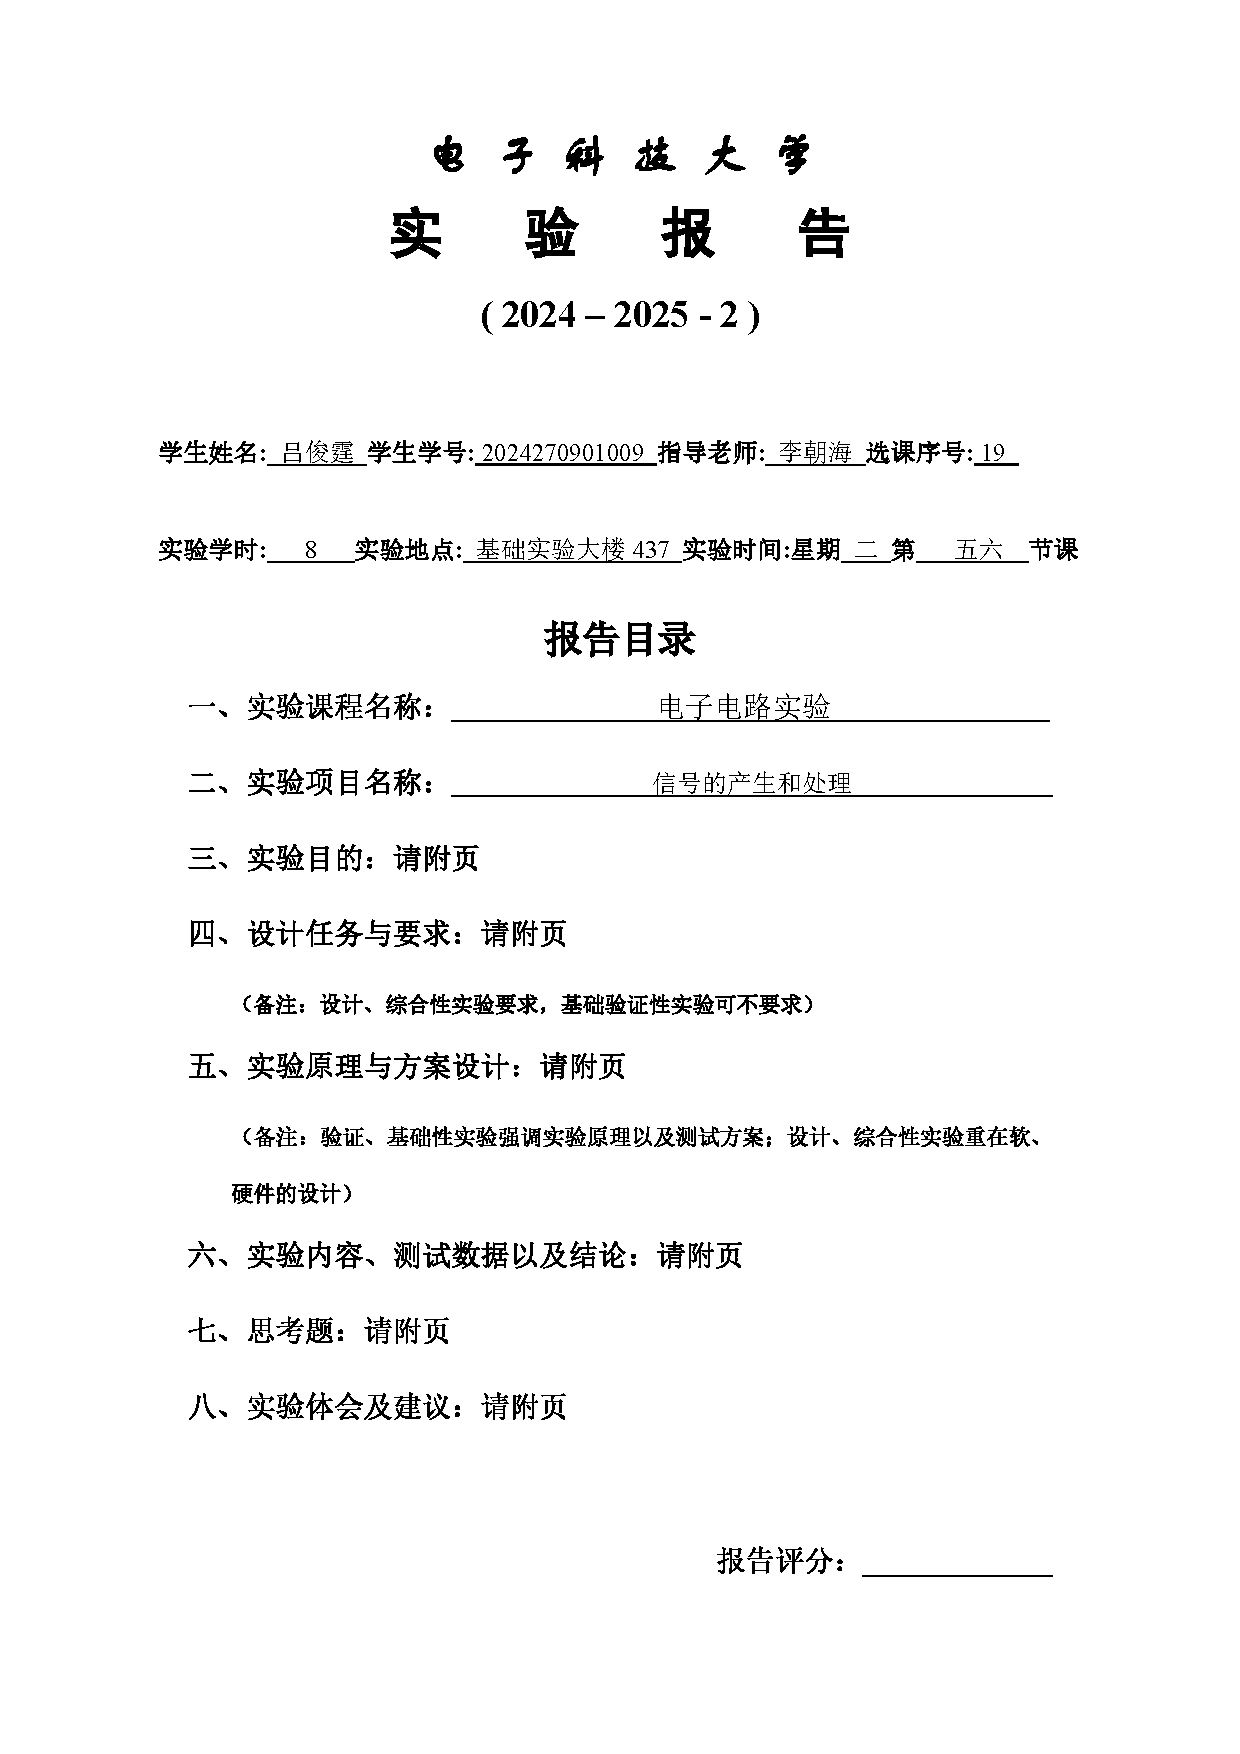
\includegraphics[page=1, width=0.9\textwidth, keepaspectratio]{image/实验报告撰写封面.pdf}
    \restoregeometry
\end{titlepage}

\setcounter{section}{2}

\clearpage
\section{实验目的}
\begin{enumerate}[leftmargin=50pt, label=(\arabic*)]
    \item 理解函数信号的产生原理
    \item 掌握利用继承运放单元电路进行电子电路系统设计的方法
    \item 掌握电路调试和指标测试技术
\end{enumerate}

\section{设计任务与要求}
用给定的运算放大器设计并制作一个信号产生与处理电路。

设计要求如图所示:设计制作一个方波产生器输出方波,再与三角波相叠加输出一个复合信号,再经过低通滤波器输出一个正弦波信号。

\begin{figure}[h]
    \centering
    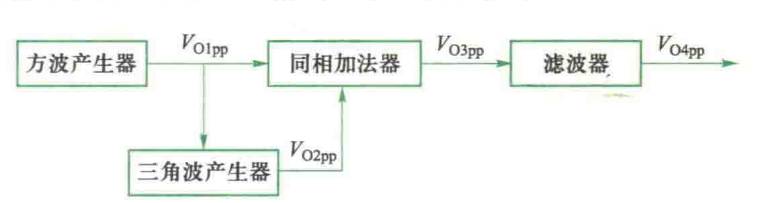
\includegraphics[width=\linewidth]{image/1.png}
    \caption{实验电路图}
    \label{fig:实验电路图}
\end{figure}

\begin{enumerate}[leftmargin=50pt, label=(\arabic*)]
    \item 方波产生器输出方波信号参数要求:$V_{o1_{pp}} = 4V$,误差为$\pm 5\%$,$f = 5\text{kHz} \pm 100\text{Hz}$;
    \item 三角波产生器输出三角波信号参数要求:$V_{o2_{pp}} = 4V$,误差为$\pm 5\%$,$f = 5\text{kHz} \pm 100\text{Hz}$;
    \item 同相加法器输出复合信号参数要求:$V_{o3_{pp}} = 8V$,误差为$\pm 5\%$,$f = 5\text{kHz} \pm 100\text{Hz}$;
    \item 滤波器输出正弦波信号参数要求:$V_{o4_{pp}} = 4V$,误差为$\pm 5\%$,$f = 5\text{kHz} \pm 100\text{Hz}$;
    \item 预留各波形的输出端口,便于后续测试;
    \item 设计报告需提供电路图、仿真及测试波形等内容。
\end{enumerate}

\clearpage
\section{实验原理与方案设计}

\subsection{实验原理}
(1) RC振荡电路
\begin{figure}[ht]
    \centering
    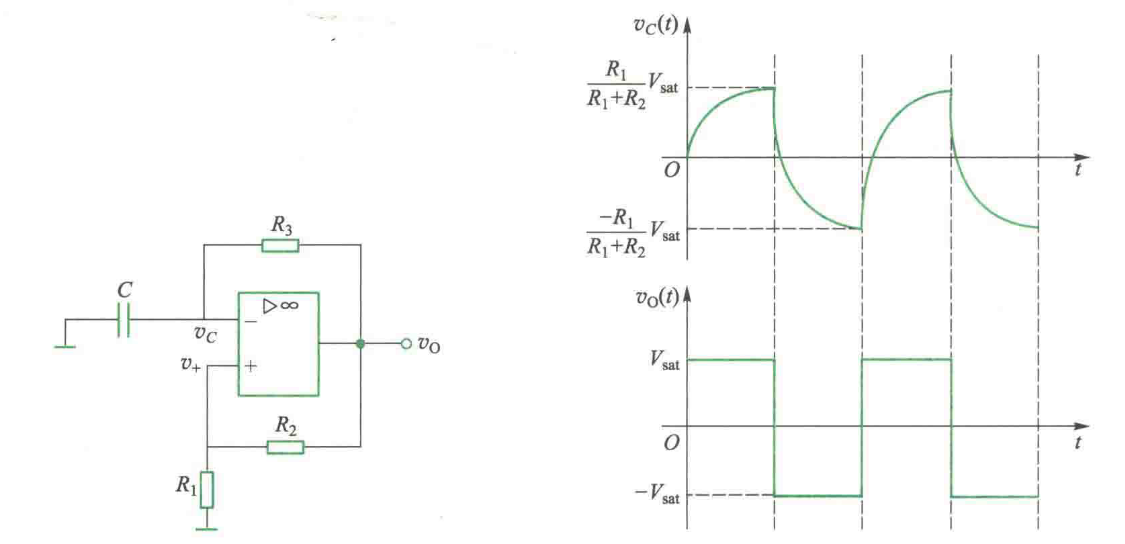
\includegraphics[width=0.6\linewidth]{image/2.png}
    \caption{RC振荡电路原理图}
    \label{fig:RC振荡电路原理图}
\end{figure}

(2) 三角波产生电路

\begin{figure}[ht]
    \centering
    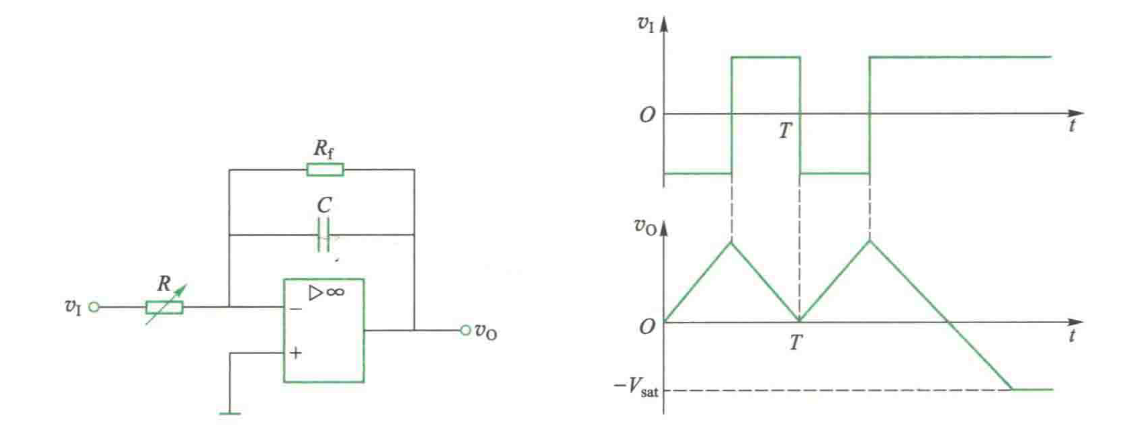
\includegraphics[width=0.6\linewidth]{image/3.png}
    \caption{三角波产生电路原理图}
    \label{fig:三角波产生电路原理图}
\end{figure}

(3) 同相加法器

\begin{figure}[ht]
    \centering
    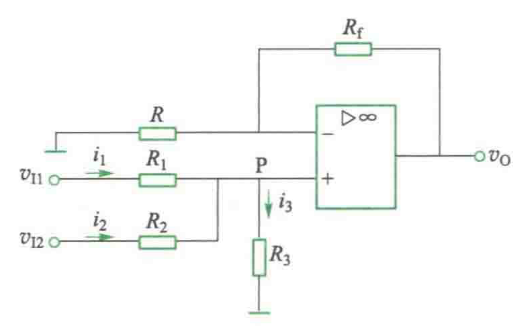
\includegraphics[width=0.6\linewidth]{image/4.png}
    \caption{同相加法器原理图}
    \label{fig:同相加法器原理图}
\end{figure}
\clearpage
(4) 滤波器

\begin{figure}[ht]
    \centering
    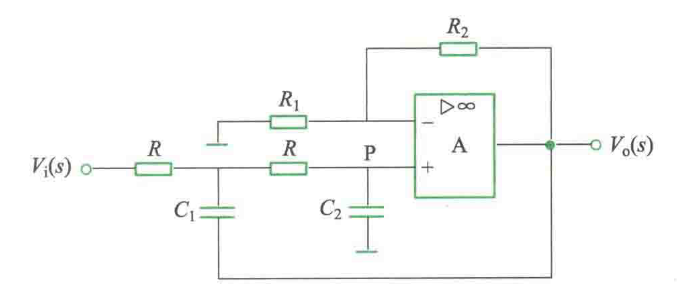
\includegraphics[width=0.6\linewidth]{image/5.png}
    \caption{滤波器原理图}
    \label{fig:滤波器原理图}
\end{figure}

\subsection{方案设计}
(此处填写你电路的设计图思路与原理框图)

\clearpage
\section{实验内容、测试数据以及结论}

\subsection{实验内容}
(简要说明接线、上电、测试流程等内容)

\subsection{实验结论}
(说明是否达到设计目标,有无失真、频率是否合格等)

\clearpage
\section{思考题}

\subsection{题面}
\begin{enumerate}[leftmargin=50pt, label=(\arabic*)]
    \item 你认为信号产生电路中运放主要起什么作用?
\end{enumerate}

\subsection{回答}
\begin{enumerate}[leftmargin=50pt, label=(\arabic*)]
    \item 运放在信号产生中起到放大、电压跟随、波形生成(积分、比较)等作用。
\end{enumerate}

\clearpage
\section{实验体会及建议}

\subsection{实验体会}
测量时应注意小心调试仪器,尽量将读数稳定在误差允许范围内进行读数。

\subsection{建议}
注意电源正负极的接入,防止反接造成仪器损坏;注意正负电压的接入,防止反接造成仪器损坏。

\end{document}
